\documentclass[10pt]{article}

\usepackage{answers}
\usepackage{setspace}
\usepackage{graphicx}
\usepackage{enumitem}
\usepackage{multicol}
\usepackage{circuitikz}
\usepackage{adjustbox}
\usepackage{mathrsfs}
\usepackage{mathtools}
\usepackage{fancyhdr}
\usepackage{svg}
\usepackage[margin=1in]{geometry}
\usepackage{amsmath,amsthm,amssymb}
\usepackage[compact]{titlesec}
\titlespacing{\section}{0pt}{*0}{-10pt}
\titlespacing{\subsection}{0pt}{*0}{-10pt}
\titlespacing{\subsubsection}{0pt}{0pt}{-10pt}
\parindent 0in
\parskip 12pt
\setlength{\headsep}{-10pt}
\setlength{\topskip}{0pt}
\setlength{\topmargin}{0pt}
\setlength{\topsep}{0pt}
\setlength{\partopsep}{0pt}
\geometry{margin=1in, headsep=0.25in}
\setlist[itemize]{label={--}, topsep=-10pt, noitemsep}
\setlist[enumerate]{topsep=-10pt, noitemsep}
\newcommand{\N}{\mathbb{N}}
\newcommand{\Z}{\mathbb{Z}}
\newcommand{\C}{\mathbb{C}}
\newcommand{\R}{\mathbb{R}}


\pagestyle{fancy}
\lhead{Aditya Arora}
\rhead{page \thepage}
\cfoot{ECE 222 Digital Computers}
\renewcommand{\headrulewidth}{0.2pt}
\begin{document}
\section*{Arithmetic}
\subsection{Full Adders ala ECE 124}
$$s_i = {x_i\oplus y_i\oplus c_i}\;\;\;; c_{i+1} = y_ic_i + x_ic_i c_iy_i$$
\subsection{Multiplication}
\subsubsection{Unsigned - Raw Multiplication}
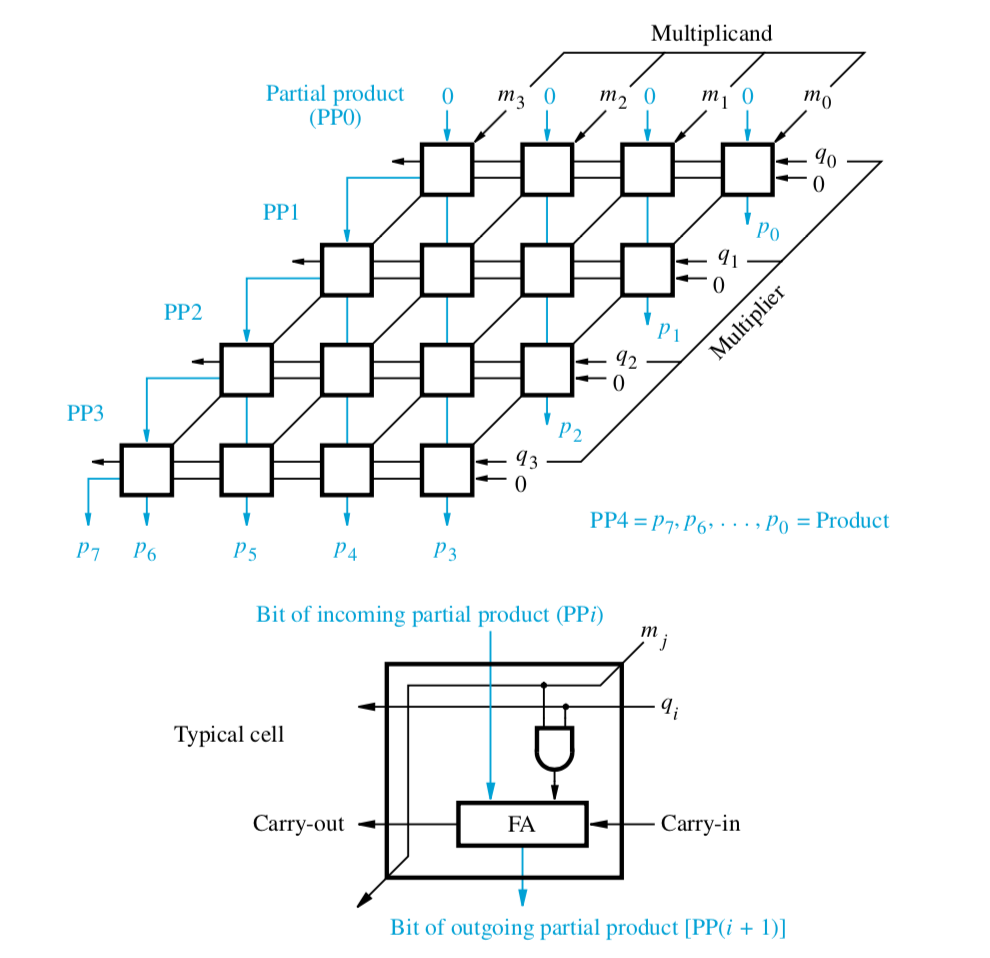
\includegraphics[width=0.8\textwidth]{arithmetic/array_multiplier.png}
\begin{itemize}
    \item Same as decimal multiplication only with ones and zeros
    \item Parts:
    \begin{itemize}
        \item Multiplicand: The number at the top
        \item Multiplier: The number at the bottom. Preferred to be the one with the fewer number of 1's
    \item The digital implementation of the raw multiplication involves a lot of cells, each with an and gate, and a full adder, alongside an input wire carrying the carry-in from the previous step
    \end{itemize}
\end{itemize}
\subsubsection{Unsigned - Sequential Multiplication}
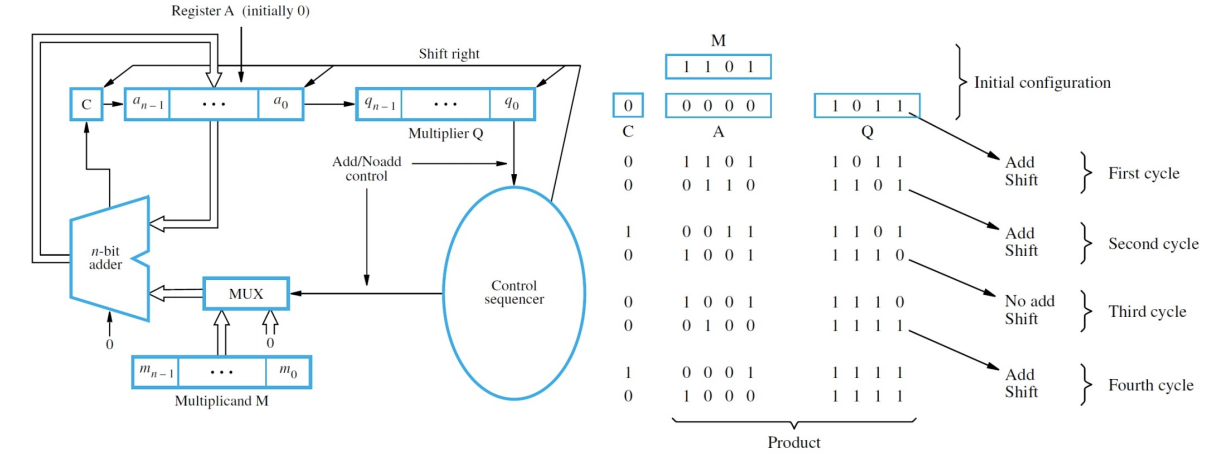
\includegraphics[width=0.8\textwidth]{arithmetic/sequential.png}
\begin{itemize}
    \item Trade-off between performance and effective resource utilization
    \item Reduce hardware replication by using a single adder, and data buffers to keep track of partial products and carrier
\end{itemize}
\subsubsection{Signed - Raw Multiplication}
Same as unsigned raw multiplication, but only with \textbf{sign extension at every stage}
\subsubsection{Signed - Booth Multiplication}
Iterate from left to right in the multiplier
\begin{enumerate}
    \item Assume there is zero to the right of the recoded number, and then proceed with normal booth recoding
    \item If there is no change in the numbers add another 0
    \item If there is a transition from 0 to 1, append $-1$
    \item If there is a transition from 1 to 0, append $1$
\end{enumerate}
After recoding the multiplier [$1\;1\;0\;1\;0 \to 0\; -1\; +1\; -1\; 0$]proceed with the multiplication as normal, when you get a -1, add the \textbf{sign extended 2's complement} of the multiplicand
\begin{itemize}
    \item If a recoded multiplier has fewer 1’s (+ve or -ve) than the original multiplier, Booth multiplication will require fewer operations. [there is no guarantee]
    \item Worst case: double the operations, Best case: just one operation
\end{itemize}
\subsubsection{Bit Pair Recoding}
Same strategy as booth algorithm's this time in groups of three. The least significant block uses only two bits of the multiplier, and assumes a zero for the third bit.\\
Again starting from the right, taking 2 bits at a time. Notice (+1 -1) is the same as (0 -1). Similarly (-1 0) is the same as (0 -2)
Just continue this to get the bit-pair recoded multiplier.\\
Proceed with multiplication as usual now, only difference being sign extension + 2's complement (for negative digit)  and shifting (for the 2's)
\newpage
\subsection{Real Numbers}
\subsubsection{Fixed Point representation}
Decimal at fixed position, same as 204.
\subsubsection{Floating Point representation}
$$F = M * \beta^E\;\;[\text{M = mantissa, E = exponent, $\beta$ = Base}]$$
It is generally assumed that the floating point numbers are normalized, i.e. the most significant digit is assumed to be 1 [saves a bit in the representation]. They can be \textit{normalized} by shifting, and \textit{denormalized} by shifting right.

Extra bits known as \textit{guard bits} are retained by floating-point
units to help preserve accuracy during arithmetic operations. The guard bits are used during normalization and rounding to preserve
the accuracy of a calculated result

In all operations we have to set NZCV status bits. The Z not only represents zero, but also stands for \textit{inexact and invalid}\\
\textit{Inexact} is the name for a result that requires rounding in order to be represented in one of the normal formats.\\
\textit{Invalid} exception occurs if operations such as 0/0 or $\sqrt{-1}$ are attempted.\\

\textbf{10.3.2.1 Single-precision  floating point representation}
$$-1^S \times q.M \times 2^{E' - 127}$$
\begin{itemize}
    \item S: 1 Sign bit
    \item E': 8 bits encoded as excess 127 i.e. E' = actual exponent - 127
    \item M: 23 bits
\end{itemize}
\textbf{10.3.2.1 Double-precision  floating point representation}
$$-1^S \times 1.M \times 2^{E' - 1023}$$
\begin{itemize}
    \item S: 1 Sign bit
    \item E': 11 bits encoded as excess 1023 i.e. E' = actual exponent - 1023
    \item M: 52 bits
\end{itemize}
\textbf{10.3.2.2 Addition and Subtraction}
\begin{enumerate}
    \item Get the two numbers to the larger exponent by shifting the one with the smaller mantissa right (this is also the exponent of the result)
    \item perform addition/subtraction on the mantissa keeping track of the sign bit
    \item Normalize the result if needed
\end{enumerate}
\textbf{10.3.2.3 Multiplication and division}\\
Multiplication:
\begin{enumerate}
    \item Add the exponents and subtract 127
    \item Multiply the mantissas and determine the sign of the result
    \item Normalize the resulting value, if necessary
\end{enumerate}
Division:
\begin{itemize}
    \item Subtract the exponents and add 127
    \item Divide the mantissas and determine the sign of the result
    \item Normalize the resulting value, if necessary\\
\end{itemize}
\newpage
\textbf{10.3.2.4 Denormalization}\\
When the value of the E’ field is 0 and M ≠ 0, a denormalized
floating-point number is represented. Denormalized numbers can be used to allow for gradual underflow and to allow for higher precision on very small values.
\begin{itemize}
    \item Single Precision Floating Point: F = $-1^S × 0.M × 2^{E’-126}$
    \item Double Precision Floating Point: $F = -1^S × 0.M × 2^{E’-1022}$
\end{itemize}
For denormalized numbers, you don't use $2^{(E - 127)}$ any more, but rather $2^{-126}$. The reasoning for this is because then there is not a gap between the smallest normal number $(1.00\dots0 \times 2^{-126})$ and the largest denormalized number $(0.111\dots1111 \times 2^{-126})$.\\

\textbf{10.3.2.5 Truncation}\\
Unbiased approximations are advantageous if many operands and operations are involved in generating a result, because positive errors tend to offset negative errors as the computation proceeds. Statistically, we can expect the results of a complex computation to be more accurate.
\begin{itemize}
    \item \underline{\textit{Chopping}}: Remove guard bits and make no changes to other bits. The result of chopping is a biased approximation because the error range is not symmetrical about 0
    \item \underline{\textit{Von Neumann rounding}}: If the bits to be removed are all 0s, they are simply dropped, with no changes to the retained bits. However, if any of the bits to be removed are 1, the least significant bit of the retained bits is set to 1. Although the range of error is larger with this technique than it is with chopping, the maximum magnitude is the same, and the approximation is unbiased because the error range is symmetrical about 0.
    \item \underline{\textit{Rounding}}: Round to the nearest number or nearest even number in case of a tie. A 1 is added to the LSB position of the bits to be retained if there is a 1 in the MSB position of the bits being removed. To break the tie in an unbiased way, one possibility is to choose the retained bits to be the nearest even number.\\
\end{itemize}

\textbf{10.3.2.6 Special Values}
\begin{table}[h!]
\begin{tabular}{l|l|l|l}
\hline
Special Value & S & E' & M \\ \hline
-0 & 1 & 0 & 0 \\
+0 & 0 & 0 & 0 \\
$-\infty$ & 1 & 255 & 0 \\
$+\infty$ & 1 & 255 & 0 \\
Denormalized value & X & 0 & M$\neq$0 \\
NaN & X & 255 & M$\neq$0
\end{tabular}
\end{table}
\end{document}
